\section{Methodology}
The first phase would involve the task of locating any object with a transceiver attached to it. We would most probably use a ultrasonic transceiver to first measure the distance of the asset to be located from three predefined coordinates we like. With the three distances in hand we can use trilateration to find the coordinate of the asset.

The second phase would be to apply this system to automate the license trial system prevalent  in Nepal. We would attach a ultrasonic transceiver with the vehicle and let it go in the track. With the coordinate of the vehicle during the course of its trial, we can calculate velocity\footnote{Calculating the derivative of the position coordinates with interpolation would give us the velocity} and acceleration in real time and report errors if any. 

We would build a \gls{gui} to display the graphical model of the real time situation. We can further save the data acquired in the server and keep for future investigation. Each of these is explained below.

\subsection{Measurement of distance}
There are various methods implemented for distance measurement electrically. Each of the methods can be implemented electrically using various component but regardless the component used, the technique remain the same. Some of the techniques are:
\subsubsection{\gls{toa}}
With TOA, the distance between the transmitting node and the receiving node is deduced from the transmission time delay and the corresponding speed of signal as follows:
\begin{equation}
	R = speed \times Time
\end{equation}
where speed denotes the traveling speed of the signal, time the amount of time spent by the signal travelling from the transmitting to the receiving node, and R the distance between the transmitting node and the receiving node. Since speed can be regarded as a known constant, R can be computed by observing time.\cite{1003.1833}

\subsubsection{\gls{tof}}
In time of flight method the time taken by signal to go from one node to the other is calculated and is used to calculate the distance. The distance can be known form the following relation.
\begin{equation}
	R = \frac{t_{rt} \times speed}{2}
\end{equation}
where $t_{rt}$ is the round trip time of the signal travel.

\subsubsection{\gls{aoa}} 
With respect to \gls{aoa} based techniques , the reference nodes or the target node has the capability of measuring the angle of arrival based on information obtained. For this purpose, techniques like angle diversity may be utilized in order to exploit the directionality of the receiver. Usually, direction finding can be accomplished by either with directional antennas or with an array of antennas. The main  principle behind the \gls{aoa} measurement via antenna arrays consists in that differences in arrival times of an incoming signal at different antenna elements include the angle information given that the array geometry is known. With \gls{aoa}, no time synchronization between nodes is required.\cite{1003.1833}
\subsection{Trilateration}
Trilateration is the technique utilized to find the co-ordinate of any point with the distance of the point given from fixed known points.	

\begin{figure}[htpb]
	\centering
	\scalebox{.4}{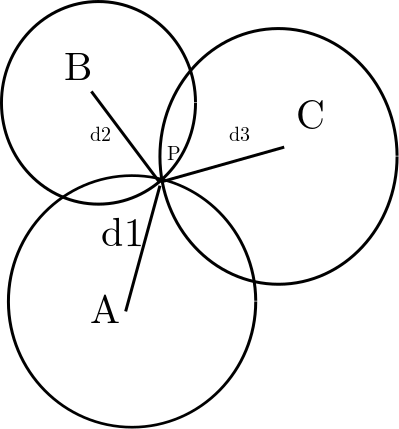
\includegraphics{./Images/Trilateration.png}}
	\caption{Trilateration}
	\label{fig:Trilateration}
\end{figure}
If in figure \ref{fig:Trilateration} the Point to be located is $P$ and the distance of $P$ from $A$ ,$B$ and $C$ is known respectively to be $d_1$, $d_2$, and $d_3$ to us.If we know the coordinate of the points $A(x_1,y_1,z_1)$ ,$B(x_2,y_2,z_2)$ and $C(x_3,y_3,z_3)$ then the coordinate $(x,y,z)$ of the point $P$ can be calculated from the set of equations:

\begin{eqnarray*}
	(x-x_1)^2+(y-y_1)^2+(z-z_1)^2 &=& d_1^2\\
	(x-x_2)^2+(y-y_2)^2+(z-z_2)^2 &=& d_2^2\\
	(x-x_3)^2+(y-y_3)^2+(z-z_3)^2 &=& d_3^2\\			
\end{eqnarray*} 
	Solving these three equation provides us with the coordinate of the point.
	\subsection{Control/Notification}
		As soon as the vehicle stops at unallowed locations in the track, or if it moves in the position to be stopped, an immediate notification will be given to the driver and s/he will be disqualified from further license processing as per the rules of Vehicle Management Department, Government of Nepal.

	\subsection{Storage to server for future use}
		The system retrives the location of the vehicle in real time. Then the data of position of vehicle can be stored in any electronic retrival media. Some dedicated server can be set up to store the data of every person who gave trial. The data can be used for future retrival for inspection or even for research purposes to find out the correlation of the data aquired with the driver.  
	\subsection{Graphical user interferance}
		With the real time data of location of the vehicle fed to the computer, we will make a visualisation showing the location of vehicle in the track and the information of the situation(speed, etc). A computer program will be made for the visualization. 
